\section{Method}
\label{sec:method}

\begin{figure*}[t]
  \centering
  % Pipeline figure (TikZ, explicit grid in cm). Orange = our additions or changes to the reference recipe.
\begin{tikzpicture}[
    font=\scriptsize, >={Stealth[length=4pt]},
    box/.style={draw=black!55, rounded corners=2pt, fill=base, align=flush center, inner sep=2.5pt, line width=0.4pt},
    ours/.style={box, draw=oursline, fill=oursfill, line width=0.6pt},
    lbl/.style={align=flush center, inner sep=1pt, text=black!75},
    arr/.style={->, line width=0.5pt, draw=black!70},
  ]
  % input, preprocessing, augmentation
  \node[inner sep=0pt] (in) at (0.8, 0.1) {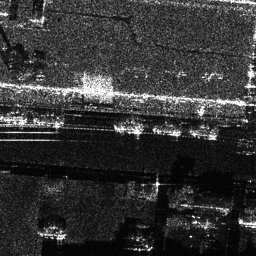
\includegraphics[width=1.5cm]{figs/thumb_input.png}};
  \node[lbl, below=0.4mm of in] {SAR image\\(gray, $\le$\,512 px)};
  \node[box, text width=1.5cm] (pre) at (2.78, 0.1) {resize 512$^2$,\\SAR mean/std,\\gray as RGB};
  \node[ours, text width=3.45cm] (aug) at (1.95, 1.72)
    {\textbf{SAR photometric augmentation}\\speckle $x\sqrt{G}$, $G{\sim}\Gamma(L,\tfrac1L)$, $L{\in}[4,16]$\\gamma $x^{\gamma}$, $\gamma{\in}[\tfrac23,\tfrac32]$ (log-uniform)\\each with $p{=}0.8$ (training only)};
  \draw[arr] (in) -- (pre);
  \draw[arr, draw=oursline] (aug.south -| pre.north) -- (pre.north);
  % shared trunk
  \node[box, minimum width=3.15cm, minimum height=2.5cm] (trunk) at (5.55, 0.2) {};
  \node[lbl, anchor=north, text=black] at (trunk.north) {\textbf{Shared trunk}: YOLO26-L\\backbone + neck};
  \node[lbl, anchor=south] at (trunk.south) {COCO-pretrained,\\26.19\,M params, all trained};
  \foreach \x/\s/\t in {4.62/0.72/{P3 (stride 8)}, 5.52/0.52/{P4 (16)}, 6.32/0.36/{P5 (32)}} {
    \node[draw=black!50, fill=white, minimum width=\s cm, minimum height=\s cm, inner sep=0pt] (f) at (\x, 0.25) {};
    \node[lbl, font=\tiny] at (\x, -0.32) {\t};
  }
  \draw[arr] (pre) -- (pre -| trunk.west);
  % heads
  \node[ours, text width=2.6cm] (cls) at (8.95, 0.82)
    {\textbf{Classification head}\\GAP(P5), LN, Linear\\$z\in\mathbb{R}^9$ (5.6\,k params)};
  \node[box, text width=2.6cm] (det) at (8.95, -0.62)
    {\textbf{Detection heads}\\one-to-many, one-to-one\\boxes $b_n$, scores $s_{n,c}$};
  \draw[arr] (trunk.east |- cls.west) -- (cls.west);
  \draw[arr] (trunk.east |- det.west) -- (det.west);
  % cross-task decoding
  \node[ours, text width=3.25cm] (fuse) at (12.55, 0.86)
    {\textbf{Detector $\to$ class} (ours)\\$\hat z_c=\log\mathrm{softmax}(z)_c$\\$\qquad+\,\beta\log\max_n s_{n,c}$};
  \node[ours, text width=3.25cm] (jd) at (12.55, -0.66)
    {\textbf{Class $\to$ detector} (ours)\\$s'_{n,c}=s_{n,c}\,\hat p_c^{\,\alpha}$, $\hat p=\mathrm{softmax}(\hat z)$\\per-class NMS 0.8, top 100};
  \draw[arr] (cls.east) -- (cls.east -| fuse.west);
  \draw[arr] (det.east) -- (det.east -| jd.west);
  \draw[arr, draw=oursline] (det.north east) -- node[lbl, left=-1pt, font=\tiny, text=oursline, pos=0.55] {$s$}
    (fuse.south west);
  \draw[arr, draw=oursline] ($(fuse.south)+(1.0,0)$) -- node[lbl, right=0pt, font=\tiny, text=oursline] {$\hat p$}
    ($(jd.north)+(1.0,0)$);
  % output
  \node[inner sep=0pt] (out) at (15.4, 0.1) {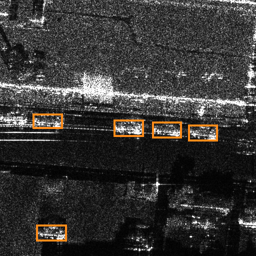
\includegraphics[width=1.5cm]{figs/thumb_output.png}};
  \node[lbl, below=0.4mm of out] {class $\arg\max\hat z$\\+ boxes (one pass)};
  \draw[arr] (fuse.east) -- (out.north west);
  \draw[arr] (jd.east) -- (out.south west);
  % training
  \node[box, fill=white, text width=11.0cm] (train) at (5.75, -2.02)
    {\textbf{Training}: $\mathcal{L}=\mathrm{CE}(z,y)+\mathcal{L}_\text{det}$ (YOLO26 box + class losses on both heads);
     h/v flips; AdamW, lr $5{\times}10^{-4}$, batch 16, cosine, EMA 0.9998, bf16, 350 epochs on all 9{,}392 train images};
  \node[ours, text width=3.95cm] (swa) at (14.0, -2.02)
    {\textbf{SWA} (ours): 12 more epochs at\\lr $5{\times}10^{-5}$, average of the\\12 epoch-end weights};
  \draw[arr] (train) -- (swa);
  % legend
  \node[ours, minimum width=3mm, minimum height=2mm, inner sep=0pt] (lg) at (0.3, -2.72) {};
  \node[lbl, anchor=west] at (0.5, -2.72) {our additions or changes};
  \node[box, minimum width=3mm, minimum height=2mm, inner sep=0pt] (lg2) at (3.25, -2.72) {};
  \node[lbl, anchor=west] at (3.45, -2.72) {standard components};
\end{tikzpicture}

  \vspace{-1mm}
  \caption{\textbf{Our pipeline.} One YOLO26-L trunk feeds a 5.6\,k-parameter classification head and YOLO26's two
  detection heads, trained jointly. Orange marks what we added or changed: SAR photometric augmentation in training,
  cross-task decoding at inference (the detector refines the image class, the class re-ranks the boxes), and SWA after
  training. Inference is one forward pass of one model.}
  \label{fig:pipeline}
\end{figure*}

\Cref{fig:pipeline} shows the pipeline.
We start with how we validate, since every later choice was made with it.

\subsection{Validation that mirrors the leaderboard}
\label{sec:protocol}
Val and test labels are hidden, so decisions are made on held-out training images.
An earlier design of ours built a leak-free holdout (LF, 940 images) that keeps near-duplicate groups whole and leaves
their neighbours out of training.
On LF the reference scores mAP 12.5 against 26.1 on val, and two candidate models swapped places between LF and val:
val rewards something LF cannot see.
We therefore select on \textbf{ND}, a stratified random 10\,\% (class\,$\times$\,image size) of the remaining training
images: 805 images, 66.5\,\% with a partner in the 7{,}252-image local train, as val images have in train.
LF (generalisation) and \textbf{FIT} (373 local-train images: fitting) are scored alongside.
Local $\Delta_m$ uses the val reference (macro-F1 93.31, mAP 26.13):
\begin{equation}
  \Delta_m=\tfrac{100\%}{2}\Big[\tfrac{\mathrm{F1}-\mathrm{F1}_\text{ref}}{\mathrm{F1}_\text{ref}}
  +\tfrac{\mathrm{mAP}-\mathrm{mAP}_\text{ref}}{\mathrm{mAP}_\text{ref}}\Big],
  \label{eq:dm}
\end{equation}
so one mAP point is worth 1.9 $\Delta_m$ and one F1 point 0.54.
A configuration is screened with one seed and decided on three, then retrained on all 9{,}392 images for submission.

\subsection{Shared-trunk multi-task model}
\label{sec:model}
The trunk is YOLO26-L~\cite{jocher2026yolo26} with COCO weights~\cite{lin2014coco}: a CSP backbone ending in an
attention block (C2PSA) at stride 32, and a neck giving P3--P5 at strides 8--32.
All 26.19\,M parameters are trained; the reference trains 21.0\,M of a 107\,M model.
The gray 512$\times$512 input (the baseline's geometry and SAR normalisation) is mapped to $[0,1]$ and repeated on
three channels, as the COCO weights expect.
\textbf{Detection:} YOLO26's one-to-many head (task-aligned assignment~\cite{feng2021tood}, NMS at inference) and
NMS-free one-to-one head predict, at each of $N{=}5{,}376$ anchor points, a box $b_n$ and class scores
$s_{n,c}\in[0,1]$; $\mathcal{L}_\text{det}$ is YOLO26's box and class loss on both heads, the one-to-many weight decaying
from 0.8 to 0.1.
\textbf{Classification:} $z=W\,\mathrm{LN}(\mathrm{GAP}(F_5))+b\in\mathbb{R}^9$ on the backbone's stride-32 feature
$F_5$ (512 channels; 5{,}641 parameters), the reference's head design.
The loss is $\mathcal{L}=\mathrm{CE}(z,y)+\mathcal{L}_\text{det}$.
A head reading P3--P5 classified better (+0.6 F1) but its gradients cost 2.1 mAP, so we kept the plain one.

\subsection{SAR photometric augmentation}
\label{sec:aug}
Besides flips, each training image $x\in[0,1]$ (amplitude) receives, each with probability $p{=}0.8$, extra speckle
\begin{equation}
  x\leftarrow x\sqrt{G},\quad G\sim\Gamma\big(L,\tfrac1L\big)\ \text{per pixel},\quad L\sim\mathcal{U}[4,16],
  \label{eq:speckle}
\end{equation}
an $L$-look intensity noise of mean 1~\cite{argenti2013speckle}, and a gamma $x\leftarrow x^{\gamma}$ with
$\log\gamma\sim\mathcal{U}[\log\tfrac23,\log\tfrac32]$.
The first mimics a revisit of the scene, the second the different intensity mappings of the source datasets.
Neither moves a pixel, so boxes stay exact and repeated scenes stay recognisable, unlike zoom and mosaic.

\subsection{Cross-task decoding}
\label{sec:decoding}
Every box of an image has the image's class, so each head holds evidence for the other, which we use at inference
with two scalars.
\emph{Detector $\to$ class:} the strongest detection of class $c$ is evidence that the image is of class $c$,
\begin{equation}
  \hat z_c=\log\mathrm{softmax}(z)_c+\beta\log\max_n s_{n,c},\qquad \hat y=\arg\max_c \hat z_c.
  \label{eq:fuse}
\end{equation}
\emph{Class $\to$ detector:} COCO AP ranks a class's boxes across all images, so boxes in an image unlikely to be of
class $c$ should rank lower,
\begin{equation}
  s'_{n,c}=s_{n,c}\,\hat p_c^{\,\alpha},\qquad \hat p=\mathrm{softmax}(\hat z).
  \label{eq:jd}
\end{equation}
Boxes come from the one-to-many head with per-class NMS at IoU 0.8; we keep the top 100 (box, class) pairs per image
with no score floor, since low-scored boxes can only add recall.
We chose $\beta{=}1$, $\alpha{=}0.5$ on ND (\cref{tab:decoding}).

\subsection{Weight averaging}
\label{sec:swa}
Training keeps an EMA of the weights (decay 0.9998).
SWA~\cite{izmailov2018swa} then continues from it for 12 epochs at a constant lr of $5{\times}10^{-5}$ and averages
the 12 epoch-end weights, batch-norm statistics included.
Averaging separately trained seeds (a model soup~\cite{wortsman2022soups}) instead collapses to $\Delta_m$ ${-}35$ to
${-}47$ on ND: the seeds end in different basins.
